\subsubsection{Scheduler Next-Event}

\begin{frame}{\subsecname: \subsubsecname}
    \begin{figure}
        \centering
        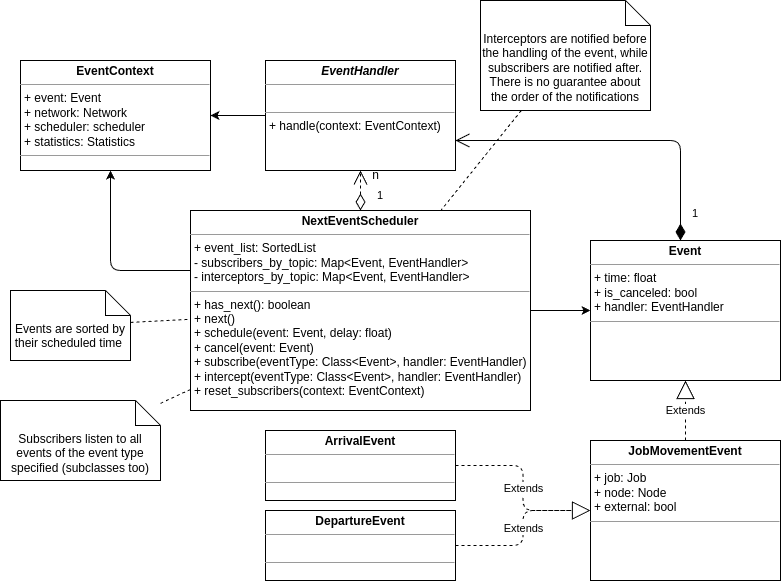
\includegraphics[width=0.7\linewidth]{figs/diagrams/scheduler.drawio.png}
        \caption{Class diagram dello scheduler Next-Event.}
        \label{fig:enter-label}
    \end{figure}
\end{frame}

\subsubsection{Event-Oriented Programming}
\begin{frame}{\subsecname: \subsubsecname}
\begin{itemize}
    \item medie calcolate secondo algoritmo di Welford \citep{des}
    \item Stimatori:
    \begin{itemize}
        \item \texttt{ArrivalsGeneratorSubscriber}
        \item \texttt{BusytimeEstimator}
        \item \texttt{ObservationTimeEstimator}
        \item \texttt{CompletionsEstimator}
        \item \texttt{ResponseTimeEstimator}
        \item \texttt{PopulationEstimator}
    \end{itemize}
    \item altri listeners:
        \begin{itemize}
            \item \texttt{ArrivalsGeneratorSubscriber}
            \item \texttt{BatchMeansInterceptor}
        \end{itemize}
\end{itemize}    
\end{frame}

\subsubsection{Job Movements}
\begin{frame}{\subsecname: \subsubsecname}
    \only<1> {\begin{figure}
        \centering
        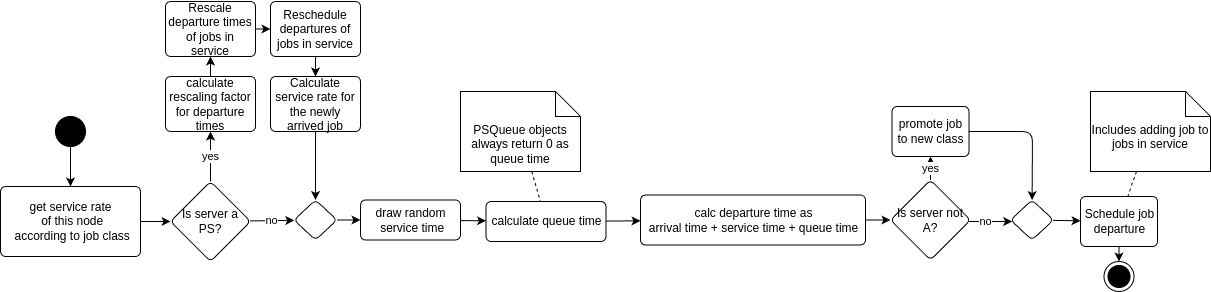
\includegraphics[width=1\linewidth]{figs/diagrams/handle_arrival_landscape.drawio.png}
        \caption{Activity diagram dell’handler degli arrivi.}
        \label{fig:enter-label}
    \end{figure}}
    \only<2> {\begin{figure}
        \centering
        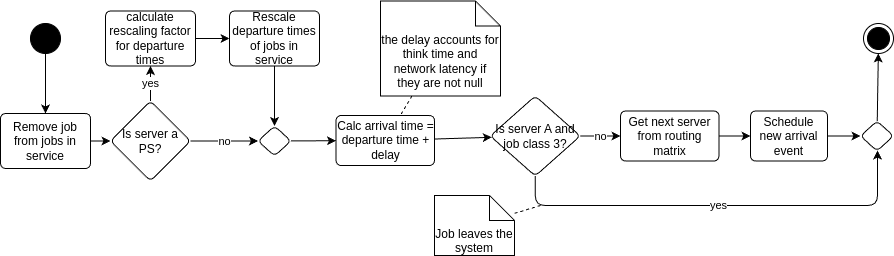
\includegraphics[width=1\linewidth]{figs/diagrams/handle_departure_landscape.drawio.png}
        \caption{Activity diagram dell’handler delle partenze.}
        \label{fig:enter-label}
    \end{figure}}    \onslide<1-> {\begin{Theorem}[Rescaled Remaining Service Time]
    \begin{equation}
      \begin{aligned}
        S^*_{rem} = S_{rem} \frac{N^*}{N}
      \end{aligned}
      \label{eq:s_rem_star_final_ps}
    \end{equation}
    \end{Theorem}}
\end{frame}

% stochastic processes
\subsubsection{Stochastic processes}
\begin{frame}{\subsecname: \subsubsecname}
    \begin{itemize}
        \item La simulazione dei processi casuali è stata implementata usando il modulo \texttt{rngs} \citep{des}
        \item Per ogni processo casuale indipendente simulato nel sistema è selezionato uno stream dedicato
        \item I processi pseudo-casuali indipendenti implementati nel sistema sono:
        \begin{itemize}
            \item  Gli arrivi dall’esterno del sistema al server A;
            \item I servizi del server A;
            \item I servizi del server B;
            \item I servizi del server P;
        \end{itemize}
    \end{itemize}
\end{frame}
% TODO: Simulation runs (BatchMeans, Replicated/Transient)

\subsubsection{Simulation Runs}
\begin{frame}{\subsecname: \subsubsecname}
    \begin{itemize}
        \item Una simulazione è implementata come un oggetto \texttt{Simulation}: \ 
        \begin{itemize}
            \item \texttt{BatchMeansSimulation}: Iscrive alla simulazione decorata un \texttt{BatchMeansInterceptor} per implementare una simulazione Batch Means;
            \item \texttt{ReplicatedSimulation}: Esegue una serie di repliche di simulazione in sequenza, impostando il seed iniziale della successiva come l'ultimo valore della sequenza prng della precedente.
        \end{itemize}
    \end{itemize}    
\end{frame}